\documentclass[12pt]{beamer}
\usetheme{Warsaw}
\usecolortheme{beaver,lily}
\usefonttheme{professionalfonts}
\setbeamertemplate{frametitle continuation}[from second][(cont.)]
\setbeamertemplate{navigation symbols}{}

\setbeamerfont{section in toc}{size=\fontsize{10}{11}\selectfont}
\setbeamerfont{subsection in toc}{size=\fontsize{8}{9}\selectfont}
\setbeamerfont{subsubsection in toc}{size=\fontsize{6}{7}\selectfont}
\setbeamercolor{section number projected}{bg=red!50!black,fg=white}
\setbeamercolor{subsection in toc}{fg=red!50!black}
\setbeamercolor{subsubsection in toc}{fg=black}
\setbeamercolor{titlelike}{fg=red!50!black}
\setbeamertemplate{subsection in toc}{
	\inserttocsubsection
	
	} % don't get rid of the above line!
\setbeamertemplate{subsubsection in toc}{
	\hspace{1.5pc}
	\textbullet\ \inserttocsubsubsection
	
	}
	
\usepackage{subfiles}
\usepackage{multicol}
\usepackage{url,hyperref}
\usepackage{tikz}
\usepackage{tkz-euclide}
%\usetkzobj{all}
\usepackage{comment}
\usepackage{enumerate}

% % %	
\begin{comment}
\AtBeginSubsection{
	\begin{frame}{}\footnotesize
	\begin{multicols}{3}
	\tableofcontents[currentsubsection,hideothersubsections]
	\end{multicols}
	\end{frame}
	}
\end{comment}	
% % %

\theoremstyle{plain}
\newtheorem{thm}{Theorem}

\theoremstyle{definition}
\newtheorem{que}{Question}
\newtheorem{ex}{Example}
\newtheorem{exe}{Exercise}
\newtheorem{dfn}{Definition}

\everymath{\displaystyle}

% % % % % % % % % %
\title[Cal III Fall 2015]{Calculus III (Math 2574)}
\subtitle{Fall 2015}
\author[Wheeler]{\footnotesize Dr. Ashley K. Wheeler}
\institute{University of Arkansas}
\date{\footnotesize{\it last updated:} \today}

% % %
\begin{document}

\frame{\titlepage}

% % %
\begin{frame}[allowframebreaks=1.00]{Table of Contents}
\begin{multicols}{3}
\tableofcontents
\end{multicols}
\end{frame}

% % % 
\section{Chapter 11}
\subsection{Week 1}
\subsubsection{Mon 24 Aug}
\begin{frame}{Mon 24 Aug}
\begin{itemize}
\item \url{http://comp.uark.edu/~ashleykw/Cal3Fall2015/cal3f15.html}
	\begin{itemize}
	\item Email me (\url{ashleykw@uark.edu}) if you did not get a message from me on Friday.
	\item ?s about the syllabus
	\end{itemize}
\item Attendance is taken using clickers.  For today, a sign-in sheet is traversing the room.  
\end{itemize}
\end{frame}

% % %
\begin{frame}{\small Tips for Success}
\begin{itemize}
\item Read. The. Textbook.
\item ``Suggested" book problems are ALL of them.  
	\begin{itemize}
	\item We may do examples in class, if there is time.  
	\item It's in your best interest to work problems that are \alert{not} in the MLP homework, then bring the ones you struggle with to drill.
	\item In the text, oftentimes there is an example, along with a list of problems covering the same concept.
	\end{itemize}
\item Play with the applets on MLP.  This course has a lot of beautiful visuals.
\item Come to office hours!  Help with topics from lecture, checking solutions to worked problems, etc.
\end{itemize}
\end{frame}

% % % 
\subsubsection{Wed 26 Aug}
\begin{frame}{Wed 26 Aug}
\begin{itemize}
\item \url{http://comp.uark.edu/~ashleykw/Cal3Fall2015/cal3f15.html}
	\begin{itemize}
	\item Email me (\url{ashleykw@uark.edu}) if you did not get a message from me on Friday.
	\item ?s about the syllabus
	\end{itemize}
\item Attendance is taken using clickers.  For today, a sign-in sheet is traversing the room.  
\item Office hours: In general, I come in between 9-10a on MWF.  However, if you need to meet earlier than that let me know in advance.
\end{itemize}
\end{frame}

% % %
\begin{frame}{}
\begin{itemize}
\item Drill section 5:30-6:20 in Ozark Hall: cancelled.  You are responsible for enrolling in a different one.  In the meantime, attend one of the following:
\begin{center}
\includegraphics[scale=0.5]{altDrills}
\end{center}
\end{itemize}
\end{frame}

% % %
\begin{frame}
\begin{itemize}
\item first MLP due Monday
\item missing lecture or drill... (transferred) Email me so you're excused.  You're responsible for the deadlines on the MLP homework.
\end{itemize}
\end{frame}

\begin{comment}
% % %
\begin{frame}
\begin{exe}[\#44 in text] In still air, a parachute with a payload would fall vertically at a terminal speed of 40 m/s.  Find the direction and magnitude of its terminal velocity relative to the ground if it falls in a steady wind blowing horizontally from west to east at 10 m/s. \end{exe}
\end{frame}
\end{comment}

% % % 
\subsubsection{Fri 28 Aug}
\begin{frame}{Fri 28 Aug}
\begin{itemize}
\item \url{http://comp.uark.edu/~ashleykw/Cal3Fall2015/cal3f15.html}
	\begin{itemize}
	\item Email me (\url{ashleykw@uark.edu}) if you did not get a message from me on Friday.
	\item ?s about the syllabus
	\end{itemize}
\item Attendance is taken using clickers STARTING MONDAY.  For today, a sign-in sheet is traversing the room.  
%\item Office hours: In general, I come in between 9-10a on MWF.  However, if you need to meet earlier than that let me know in advance.
\end{itemize}
\end{frame}

% % %
\begin{frame}
\begin{itemize}
\item first MLP due Monday
\item missing lecture or drill... (transferred) Email me so you're excused.  You're responsible for the deadlines on the MLP homework.
\item 1st Quiz: next week, likely Tuesday.  Anything from the first four sections of Chapter 11 is game.
\end{itemize}
\end{frame}

% % % 
\subsection{Week 2}
\subsubsection{Mon 31 Aug}
\begin{frame}{Mon 31 Aug}
\begin{itemize}
\item \url{http://comp.uark.edu/~ashleykw/Cal3Fall2015/cal3f15.html}
	\begin{itemize}
	\item The instructions for MLP are in the syllabus.
	\item The first homework is due tonight.  Don't wait until the last minute.
	\end{itemize}
\item Attendance is now taken using clickers. 
\item Quiz 1 tomorrow (Tuesday) in drill, 10 minutes.  Need to know definition of \alert{orthogonal}.
\end{itemize}
\end{frame}

% % %
\subsubsection{Wed 2 Sep}
\begin{frame}{Wed 2 Sep}
\begin{itemize}
\item Tips on HW
	\begin{itemize}
	\item Print and do the MLP assignment before going to book problems.
	\item Areas to review:
		\begin{itemize}
		\item setting up and solving equations, degrees of freedom
		\item completing the square and other algebra
		\item collinear points, planar geometry
		\item Chapter 10
		\end{itemize}
	\end{itemize}
\end{itemize}
\end{frame}

% % %
\subsubsection{Fri 4 Sep}
\begin{frame}{Fri 4 Sep}
\begin{itemize}
\item Clickers next week.
\item Quiz 2 on Tuesday, a little longer than Quiz 1.
\item First Exam on Friday 18 Sep.  Covers Chapter 11.  There is a chance we will skip 11.9.
\item MLP troubles: Use the list of instructions on the syllabus, or else visit the MRTC help page.
\end{itemize}
\end{frame}

\begin{frame}
\begin{itemize}
\item Tips on HW
	\begin{itemize}
	\item Print and do the MLP assignment before going to book problems.
	\item Areas to review:
		\begin{itemize}
		\item setting up and solving equations, degrees of freedom
		\item completing the square and other algebra
		\item collinear points, planar geometry
		\item Chapter 10
		\end{itemize}
	\end{itemize}
\end{itemize}
\end{frame}

\begin{frame}{\small Note-Taker Needed for 12:55 Section}\footnotesize
From the CEA Office:

%\vspace{0.5pc}
%\hspace{0.5pc}
\begin{quotation}%\alert{
A student in this class requires a note-taker. If you are willing to upload your notes and plan to attend class on a REGULAR basis, please sign up via the CEA Online Services on the Center for Educational Access (CEA) website \url{http://cea.uark.edu}. On the CEA Online Services login screen, click on ``Sign Up as a Note-taker". 
%
%\vspace{0.5pc}
At the end of the semester you will receive verification of 48 community service hours OR a \$50 gift card for providing class notes. All interested students are encouraged to sign up; preference may be given to volunteers seeking community service in an effort engage U of A students in community service opportunities. 
%
%\vspace{0.5pc}
Please contact the Center for Educational Access at \url{ceanotes@uark.edu} if you have any questions.
%}
\end{quotation}
\end{frame}

% % % % %
\subsection{Week 3}
% % %
\subsubsection{Wed 9 Sep}
\begin{frame}{Wed 9 Sep {\it \small (Wheeler absent)}}\footnotesize
\begin{itemize}
\item Read the textbook ahead of time!
\item Blackboard?
\item You may attend the other (Wheeler) section as long as your attendance is documented.  See the webpage/syllabus for the time and location.
\item Excused absences: Please email me if you know you'll be absent and why.  If relevant, provide documentation such as a doctor's note.
\item First Exam on Friday 18 Sep.  Covers Chapter 11.  There is a chance we will skip 11.9.
\item MLP troubles: Use the list of instructions on the syllabus, or else visit the MRTC help page.
\end{itemize}
\end{frame}

\begin{frame}{\small Note-Taker Needed for 12:55 Section}\footnotesize
From the CEA Office:

%\vspace{0.5pc}
%\hspace{0.5pc}
\begin{quotation}%\alert{
A student in this class requires a note-taker. If you are willing to upload your notes and plan to attend class on a REGULAR basis, please sign up via the CEA Online Services on the Center for Educational Access (CEA) website \url{http://cea.uark.edu}. On the CEA Online Services login screen, click on ``Sign Up as a Note-taker". 
%
%\vspace{0.5pc}
At the end of the semester you will receive verification of 48 community service hours OR a \$50 gift card for providing class notes. All interested students are encouraged to sign up; preference may be given to volunteers seeking community service in an effort engage U of A students in community service opportunities. 
%
%\vspace{0.5pc}
Please contact the Center for Educational Access at \url{ceanotes@uark.edu} if you have any questions.
%}
\end{quotation}
\end{frame}

% % %
\subsubsection{Fri 11 Sep}
\begin{frame}{Fri 11 Sep}
\begin{itemize}
\item Clickers: Channel 41
\item Blackboard?
\item First Exam on Friday 18 Sep.  
	\begin{itemize}
	\item Covers up to 11.8.  
	\item No calculators.
	\item Stay tuned: A list of suggested book problems will be posted on the course webpage.
	\end{itemize}
\item Quiz 3 on Tuesday, up to 11.8 is game (emphasis on curves, parametrizions, arc length).
\end{itemize}
\end{frame}

\begin{frame}[allowframebreaks]{\small Attendance Questions}
\begin{itemize}
\item Excused absences: Please email me if you know you'll be absent and why.  If relevant, provide documentation such as a doctor's note.
\item You may attend the other (Wheeler) section as long as your attendance is documented.  See the webpage/syllabus for the time and location.  BUT...
\framebreak
\item \alert{Alternate Drills:} Please do everything you can to attend your {\it scheduled} drill.
	\begin{itemize}
	\item If you don't like your scheduled drill, change it in ISIS.
	\item If you cannot change your drill then you {\it must} have permission from the instructor to attend a different drill.  If the instructor says no, then they say no (so work out the arrangement ahead of time).  You are responsible for your attendance being documented.
	\item Since there are no makeups allowed for quizzes, you are allowed to attend an alternate drill to take a quiz.  {\it Again,} you must have permission from the drill instructor (so work out the arrangement ahead of time).	
	\end{itemize}
\end{itemize}
\end{frame}

\begin{frame}[allowframebreaks]{\small Homework Questions}
\begin{itemize}
\item MLP troubles: Use the list of instructions on the syllabus, or else visit the MRTC help page.
\item Read the textbook ahead of time -- before lecture!  Then start the homework after lecture, the same day.
\item Print the MLP assignment so you're not limited to working at a computer.  
\item The problems are chosen and assigned by the Coordinator.  Expect one set per section covered.  You are responsible for meeting the deadlines.
\end{itemize}
\end{frame}

\begin{frame}{\small Note-Taker Needed for 12:55 Section}\footnotesize
From the CEA Office:

%\vspace{0.5pc}
%\hspace{0.5pc}
\begin{quotation}%\alert{
A student in this class requires a note-taker. If you are willing to upload your notes and plan to attend class on a REGULAR basis, please sign up via the CEA Online Services on the Center for Educational Access (CEA) website \url{http://cea.uark.edu}. On the CEA Online Services login screen, click on ``Sign Up as a Note-taker". 
%
%\vspace{0.5pc}
At the end of the semester you will receive verification of 48 community service hours OR a \$50 gift card for providing class notes. All interested students are encouraged to sign up; preference may be given to volunteers seeking community service in an effort engage U of A students in community service opportunities. 
%
%\vspace{0.5pc}
Please contact the Center for Educational Access at \url{ceanotes@uark.edu} if you have any questions.
%}
\end{quotation}
\end{frame}

% % % % %
\subsection{Week 4}
% % %
\subsubsection{Mon 14 Sep}
\begin{frame}{Mon 14 Sep}
\begin{itemize}
\item Clickers: Channel 41
\item Exam this Friday 18 Sep
	\begin{itemize}
	\item Covers up to 11.8.  
	\item No calculators.
	\item A list of suggested book problems is posted on the course webpage.  Don't worry about 11.9.
	\end{itemize}
\item Quiz 3 tomorrow (Tuesday), up to 11.8.  Be sure to study 11.7 as well (e.g., do the MLP).  
\end{itemize}
\end{frame}

\begin{frame}[allowframebreaks]{\small Attendance Questions}
\begin{itemize}
\item Excused absences: Please email me if you know you'll be absent and why.  If relevant, provide documentation such as a doctor's note.
\item You may attend the other (Wheeler) section as long as your attendance is documented.  See the webpage/syllabus for the time and location.  BUT...
\framebreak
\item \alert{Alternate Drills:} Please do everything you can to attend your {\it scheduled} drill.
	\begin{itemize}
	\item If you don't like your scheduled drill, change it in ISIS.
	\item If you cannot change your drill then you {\it must} have permission from the instructor to attend a different drill.  If the instructor says no, then they say no (so work out the arrangement ahead of time).  You are responsible for your attendance being documented.
	\item Since there are no makeups allowed for quizzes, you are allowed to attend an alternate drill to take a quiz.  {\it Again,} you must have permission from the drill instructor (so work out the arrangement ahead of time).	
	\end{itemize}
\end{itemize}
\end{frame}

\begin{frame}[allowframebreaks]{\small Homework Questions}
\begin{itemize}
\item MLP troubles: Use the list of instructions on the syllabus, or else visit the MRTC help page.
\item Read the textbook ahead of time -- before lecture!  Then start the homework after lecture, the same day.
\item Print the MLP assignment so you're not limited to working at a computer.  
\item The problems are chosen and assigned by the Coordinator.  Expect one set per section covered.  You are responsible for meeting the deadlines.
\end{itemize}
\end{frame}

\begin{frame}{\small Note-Taker Needed for 12:55 Section}\footnotesize
From the CEA Office:

%\vspace{0.5pc}
%\hspace{0.5pc}
\begin{quotation}%\alert{
A student in this class requires a note-taker. If you are willing to upload your notes and plan to attend class on a REGULAR basis, please sign up via the CEA Online Services on the Center for Educational Access (CEA) website \url{http://cea.uark.edu}. On the CEA Online Services login screen, click on ``Sign Up as a Note-taker". 
%
%\vspace{0.5pc}
At the end of the semester you will receive verification of 48 community service hours OR a \$50 gift card for providing class notes. All interested students are encouraged to sign up; preference may be given to volunteers seeking community service in an effort engage U of A students in community service opportunities. 
%
%\vspace{0.5pc}
Please contact the Center for Educational Access at \url{ceanotes@uark.edu} if you have any questions.
%}
\end{quotation}
\end{frame}

% % %
\subsubsection{Wed 16 Sep}
\begin{frame}{Wed 16 Sep}
\begin{itemize}
\item Clickers: Channel 41
\item Exam this Friday 18 Sep
	\begin{itemize}
	\item Covers up to 11.8.  
	\item No calculators.
	\item A list of suggested book problems is posted on the course webpage.  Don't worry about 11.9.
	\item Includes an ``open-ended" portion... Compare to the rigor of Quiz 3.  Likely to be take-home.
	\item Graded exams won't be returned until at least Monday 28 Sep.
	\end{itemize}
\item Quiz 1-3 solutions posted on MLP
\end{itemize}
\end{frame}

\begin{frame}[allowframebreaks]{\small General Study Tips}
\begin{itemize}
\item Hopefully, you've been doing those book problems.
\item Review MLP problems.  If there was a problem you got wrong the first time, do it again until you get it perfect.
\item When doing problems, write up the answers nicely.  You don't need as much detail as Quiz 3, \alert{BUT} if you were to look at your work one year from now, you should have written enough to be able to follow it.
\item Redo quizzes, too.  Only one version of each of the first two quizzes is posted, so practice with the other versions.
\framebreak
\item Review notes from class and reread (but not too slowly) the text.  If necessary, get notes from a friend on days you missed or else reread those sections more carefully.
\item Look at pictures in the book, especially any of the applets in MLP.
\item Know the special triangles.
\item Correct any lingering algebra, trig, geometry, Cal I rustiness.
\framebreak
\item Definitions
	\begin{itemize}
	\item Know ``vocabulary words", not in order to recite the definitions, but so that you can understand what a question is asking.
	\begin{ex}[s]
	\begin{enumerate}
	\item Given $\overrightarrow{r}(t)$, find the {\bf tangent vector}.
	\item {\bf smooth} vs. {\bf differentiable} (in Cal I and in Cal III)
	\item ``Parametrize..." or ``Eliminate the parameter"
	\end{enumerate}
	\end{ex}
	\end{itemize}
\framebreak
\item Formulas
	\begin{itemize}
	\item Memorize them all...
	\item \alert{OR} know a few key formulas.  Many of the others you can figure out from the context of the problem. 
	\item Some suggested key formulas:
		\begin{itemize}
		\item distance and midpoint between two given points
		\item equations for spheres and balls
		\item simple (parallel to those given by the coordinates) planes and lines
		\item both dot product formulas (and when one is more useful than the other)
		\item both projection formulas (and when one is more useful than the other)
\framebreak
		\item cross product formula and the formula for its magnitude
		\item parametrized line in $\mathbb R^3$
		\item normalization of a vector
		\item arc length
		\end{itemize}
%\framebreak
	\item Physics formulas ({\bf boldface} indicates a vector quantity):
		\begin{itemize}
		\item Work = {\bf Force} $\bullet$ {\bf displacement}
		\item {\bf torque} = {\bf radial force} $\times$ {\bf applied force}
		\item {\bf magnetic force} = (charge){\bf velocity} $\times$ {\bf magnetic field}
		\item Newton no. 2: {\bf total force} = (mass){\bf acceleration}
		\end{itemize}
	\end{itemize}
\framebreak	
\item Recognize key pictures: planes, lines, circles, helices.	
\item Know how to do calculus on vectors -- derivative rules, integrals, limits, continuity, story problems, etc.
\end{itemize}
\end{frame}

% % % % %
\section{Chapter 12}
\subsection{Week 5}
% % %
\subsubsection{Mon 21 Sep}
\begin{frame}{Mon 21 Sep}%\footnotesize
\begin{itemize}
\item About the exam...
\item MLP stay tuned
\item Quiz tomorrow, probably
\end{itemize}
\end{frame}

% % %
\begin{frame}[allowframebreaks]{\small Pictures!}{}
Graphs of functions of two variables:

\vspace{-2.75pc}
\begin{center}
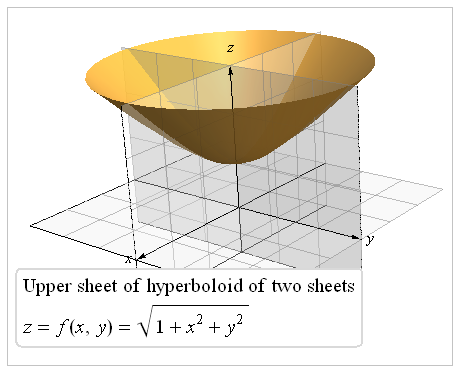
\includegraphics[scale=0.45]{12-2functionsHyp}
\hfill
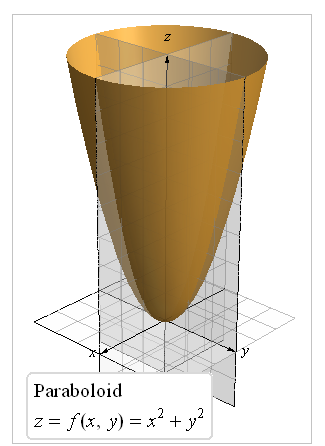
\includegraphics[scale=0.45]{12-2functionsParab}
\end{center}

\vspace{-1pc}
\hfill{\footnotesize (See the interactive pictures in MLP.)}

\framebreak
Level Curves v. Contour Curves
\begin{center}
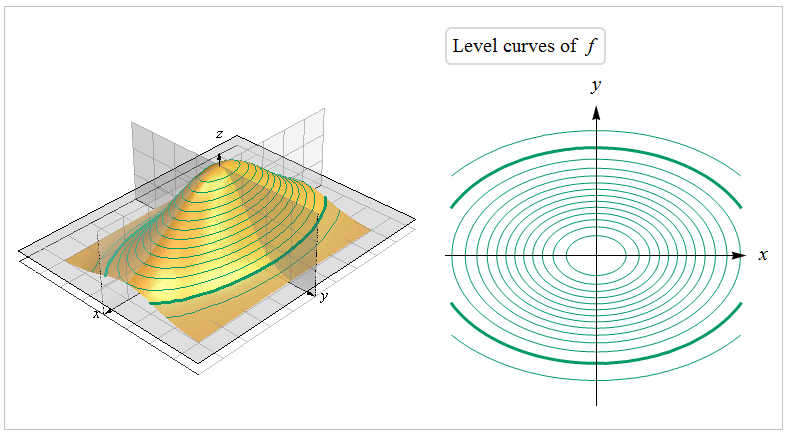
\includegraphics[scale=0.45]{12-2levCurves}
\end{center}

\framebreak
\begin{center}
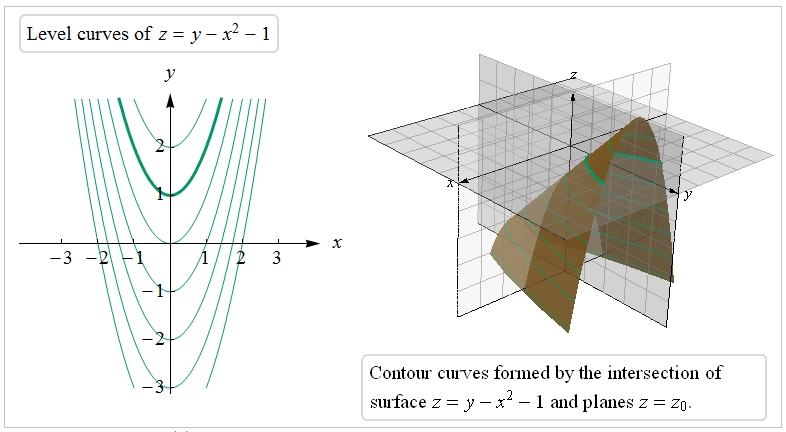
\includegraphics[scale=0.5]{12-2levCurves2}
\end{center}

\framebreak
%\footnotesize \tiny 
Application: \tiny
\vspace{-0.75pc}

\begin{center}
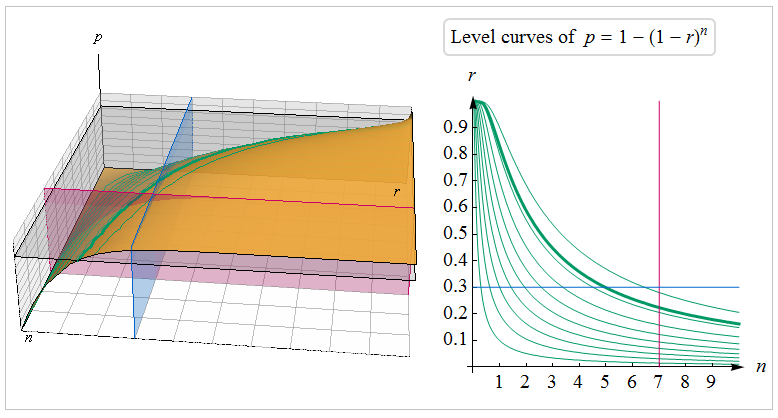
\includegraphics[scale=0.4]{12-2levCurvesAppl}
\end{center}
\vspace{-1pc}
\[\begin{split}
r &=\text{fraction of sick students who took the Exam last Friday} \\
n &= \text{number of tests Wheeler has graded so far} \\
p(n,r) &=\text{probability Wheeler graded an infected test}
\end{split}\]
\end{frame}

% % %
\subsubsection{Wed 23 Sep}
\begin{frame}{Wed 23 Sep}%\footnotesize
\begin{itemize}
\item Preliminary exam feedback.
\item MLP homeworks for Chapter 12 are posted.
\item Exam 2 is in 3 weeks.
	\begin{itemize}
	\item Be proactive!  Read ahead, do the homework as soon as possible.  DON'T SKIP CLASS.
	\item Follow instructions.  On Quizzes, on the Exam, etc.
	\item Fix your algebra, trig, Cal I-II.
	\end{itemize}
\end{itemize}
\end{frame}

%
\begin{frame}{\small Running out of time on the Exam}\footnotesize
Budget your time.  Here is a strategy that worked for me:
\begin{itemize}
\item[1. ] Count the problems.  Exam 1 had 7 problems.  With 50 minutes, each problem should take no more than 7 minutes.
\item[2. ] If there is an obivously easy problem, do it first.  Otherwise, go through the entire exam, spending up to 3 minutes per problem.  Some problems you will finish, some you won't.
\item[3. ] Of the problems you didn't finish, go back and prioritize according to those you think you know how to answer.
\item[4. ] When you get to the point where you are still stumped, check your work on the problems you did answer.
\item[5. ] Repeat Step 3. 
\end{itemize}
\end{frame}

%
\begin{frame}{\small Picture!}\footnotesize
Example of Two-Path Test:
\begin{center}
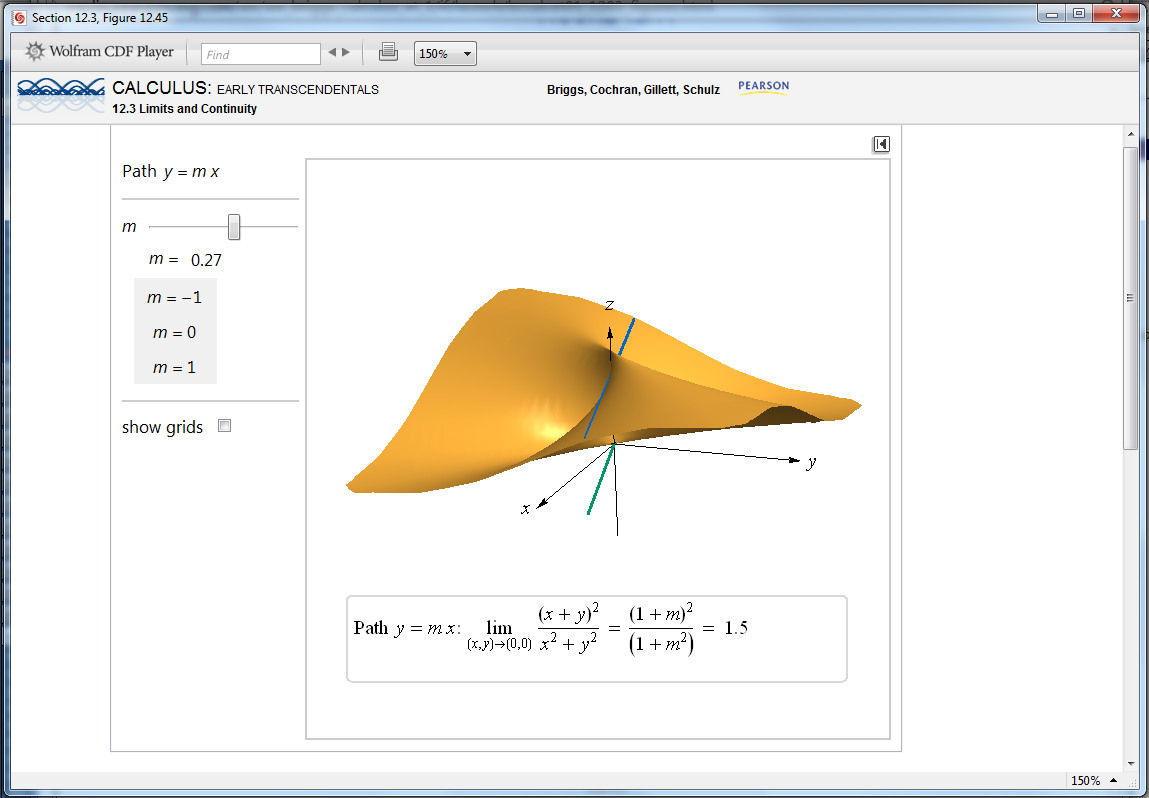
\includegraphics[scale=0.27]{12-3twoPathTest}
\end{center}
\end{frame}

% % %
\subsubsection{Fri 25 Sep}
\begin{frame}{Fri 25 Sep}%\footnotesize
\begin{itemize}
\item Quiz on Tuesday, \underline{probably}.
\item Exam feedback:

\vspace{0.5pc}
\includegraphics[scale=0.85]{exam1Medians}
	\begin{itemize}
	\item Curve: TBD.  Wheeler average was 6 points lower than VHM (Coordinator).
	\end{itemize}
\end{itemize}
\end{frame}

%
\begin{frame}
\begin{itemize}
\item Exam 2 is Wed 14 Oct.
	\begin{itemize}
	\item Be proactive!  Read ahead, do the homework as soon as possible.  DON'T SKIP CLASS.
	\item Follow instructions.  On Quizzes, on the Exam, etc.
	\item Fix your algebra, trig, Cal I-II.
	\item Drill: Don't let the drill instructor choose problems for you.  Bring questions to ask at the beginning of class.  If the problem is a little different from MLP, email them in advance (or go to office hours).
	\item Shortcuts on problems/showing work: Bring your practice problems to office hours.
	\end{itemize}
\end{itemize}
\end{frame}

% 
\begin{frame}{\small Picture!}\footnotesize
$f$ is not continuous nor differentiable at $(0,0)$... but both partial derivatives exist!
\begin{center}
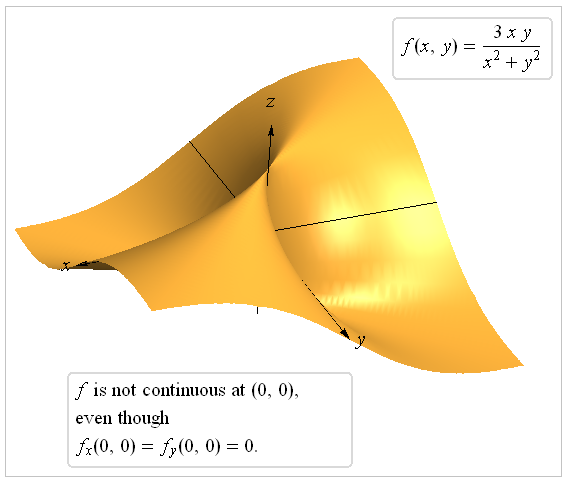
\includegraphics[scale=0.4]{12-4diff}
\end{center}
\end{frame}

% % % % %
\subsection{Week 6}
% % %
\subsubsection{Mon 28 Sep}
\begin{frame}{Mon 28 Sep}%\footnotesize
\begin{itemize}
\item Quiz on Tuesday, \underline{probably}.  Up to 12.4 is game.
\item Exam feedback:

\vspace{0.5pc}
\includegraphics[scale=0.85]{exam1Medians}
	\begin{itemize}
	\item Curve: TBD.  Wheeler average was 6 points lower than VHM (Coordinator).
	\end{itemize}
\end{itemize}
\end{frame}

%
\begin{frame}
\begin{itemize}
\item Exam 2 is Wed 14 Oct.
	\begin{itemize}
	\item Be proactive!  Read ahead, do the homework as soon as possible.  DON'T SKIP CLASS.
	\item Follow instructions.  On Quizzes, on the Exam, etc.
	\item Fix your algebra, trig, Cal I-II.
	\item Drill: Don't let the drill instructor choose problems for you.  Bring questions to ask at the beginning of class.  If the problem is a little different from MLP, email them in advance (or go to office hours).
	\item Shortcuts on problems/showing work: Bring your practice problems to office hours.
	\end{itemize}
\end{itemize}
\end{frame}

% % %
\subsubsection{Wed 30 Sep}
\begin{frame}{Wed 30 Sep}%\footnotesize
\begin{itemize}
\item Quiz next week (on Tuesday), covers 12.4-12.6.  
\item Exam 1 Curve: Everyone gets 6 more points.
\item MLP: up to 12.5 is now posted...
\end{itemize}
\end{frame}

%
\begin{frame}
\begin{itemize}
\item Exam 2 is Wed 14 Oct.
	\begin{itemize}
	\item Be proactive!  Read ahead, do the homework as soon as possible.  DON'T SKIP CLASS.
	\item Follow instructions.  On Quizzes, on the Exam, etc.
	\item Fix your algebra, trig, Cal I-II.
	\item Drill: Don't let the drill instructor choose problems for you.  Bring questions to ask at the beginning of class.  If the problem is a little different from MLP, email them in advance (or go to office hours).
	\item Shortcuts on problems/showing work: Bring your practice problems to office hours.
	\end{itemize}
\end{itemize}
\end{frame}

% % %
\subsubsection{Fri 2 Oct}
\begin{frame}{Fri 2 Oct}%\footnotesize
\begin{itemize}
\item Quiz next week (on Tuesday), covers 12.4-12.6.  
\item Exam 1 Curve: Everyone gets 6 more points.  Stay tuned for solutions.
\item MLP will be fixed by the end of the day today.
\end{itemize}
\end{frame}

%
\begin{frame}
\begin{itemize}
\item Exam 2 is Wed 14 Oct.
	\begin{itemize}
	\item Be proactive!  Read ahead, do the homework as soon as possible.  DON'T SKIP CLASS.
	\item Follow instructions.  On Quizzes, on the Exam, etc.
	\item Fix your algebra, trig, Cal I-II.
	\item Drill: Don't let the drill instructor choose problems for you.  Bring questions to ask at the beginning of class.  If the problem is a little different from MLP, email them in advance (or go to office hours).
	\item Shortcuts on problems/showing work: Bring your practice problems to office hours.
	\end{itemize}
\end{itemize}
\end{frame}

% % % % %
\subsection{Week 7}
% % %
\subsubsection{Mon 5 Oct}
\begin{frame}{Mon 5 Oct}%\footnotesize
\begin{itemize}
\item Quiz tomorrow 12.4-12.6.
\item Exam 1 Solutions posted to MLP.  Top right corner under ``Doc Sharing".
\item MLP should be fixed now.
\item Exam 2 is next week.
\end{itemize}
\end{frame}

%
\begin{frame}[allowframebreaks]{\small Pictures! and Links!}\tiny
{\footnotesize Linear Approximation: Cal I v. Cal III}
\vspace{-1pc}
\begin{center}
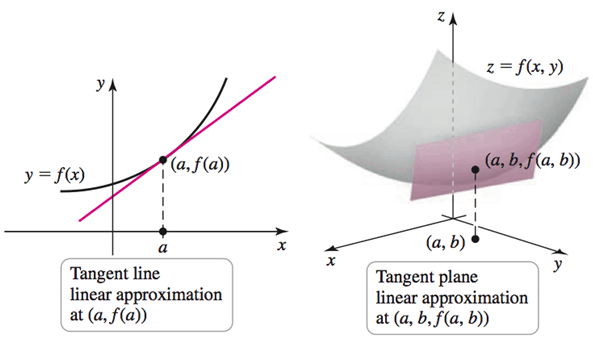
\includegraphics[scale=0.5]{12-7linApprox}
\end{center}
%
\framebreak
{\footnotesize Differentials}
\vspace{-1.5pc}
\begin{center}
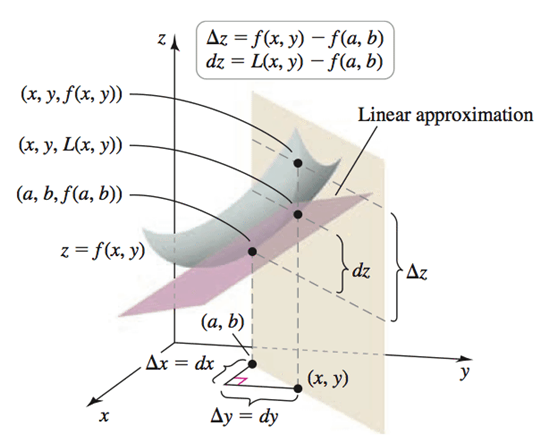
\includegraphics[scale=0.45]{12-7differentials}
\end{center}
%
\framebreak
\begin{center}
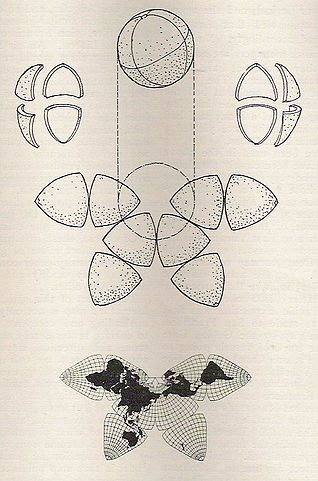
\includegraphics[scale=0.6]{318px-Cahill_Butterfly_Map}

\href{https://en.wikipedia.org/wiki/Bernard_J._S._Cahill} {Cahill Butterfly Map}. 

Image licensed under Public Domain via \href{https://commons.wikimedia.org/wiki/}{Commons}.
\end{center}
%
\framebreak
\begin{center}
\href{https://en.wikipedia.org/wiki/Cahill-Keyes_projection}{
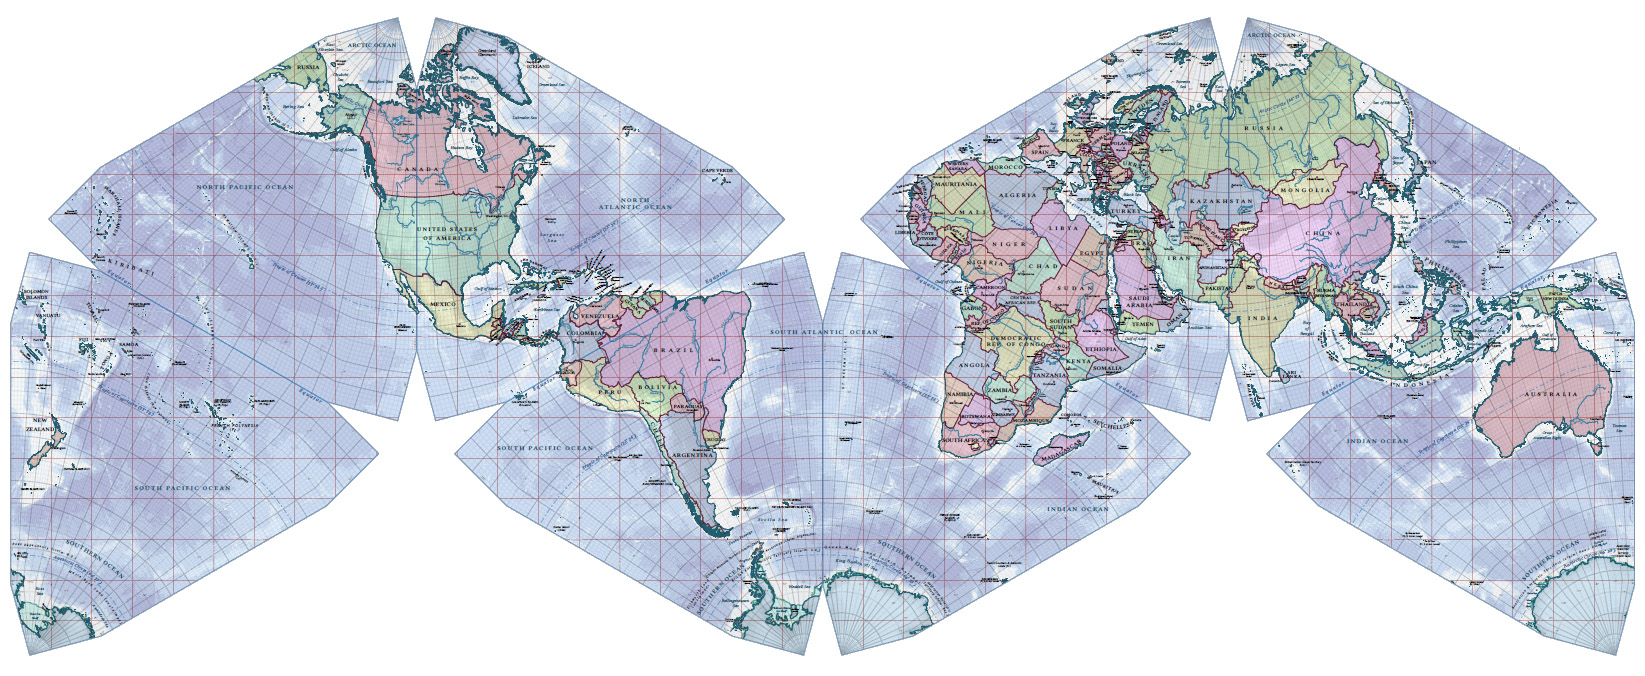
\includegraphics[scale=0.18]{World_Map,_Political,_2012,_Cahill-Keyes_Projection}
}

``World Map, Political, 2012, Cahill-Keyes Projection" by Duncan Webb - Provided by author via e-mail.. 

Licensed under CC BY 1.0 via Commons
\end{center}
%
\framebreak
\begin{center}
\href{https://en.wikipedia.org/wiki/Dymaxion_map}{

\includegraphics[scale=0.4]{640px-Dymaxion_map_ocean2}
}

\vspace{0.5pc}
``Dymaxion map ocean2" by Based on en:File:Dymaxion\_map\_unfolded.png. 

Licensed under CC BY 2.5 via Commons
\end{center}
\end{frame}

% % %
\subsubsection{Wed 7 Oct}
\begin{frame}{Wed 7 Oct}%\footnotesize
\begin{itemize}
\item Quiz tomorrow 12.4-12.6.  No quiz next week but there is one the Thursday after Fall Break.
\item Exam 2 is next week.
	\begin{itemize}
	\item $\sim$7 questions
	\item Get comfortable with ``gnarly" computations.  The best way is to show work while practicing.  See Exam 1 solutions for other shortcuts in work.
	\item No calculators.  
	\item Takehome in drill on Tuesday, covers $\textstyle\oint$12.9.
	\item Expect a list of book problems this weekend.
	\end{itemize}
\end{itemize}
\end{frame}

% 
\begin{frame}[allowframebreaks]{\small Pictures!}
\begin{center}
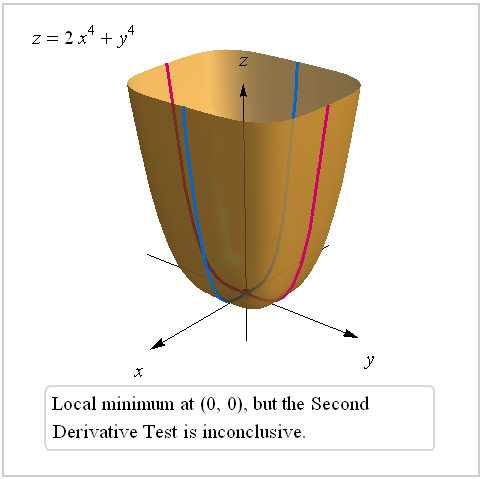
\includegraphics[scale=0.4]{12-8inconclusive}
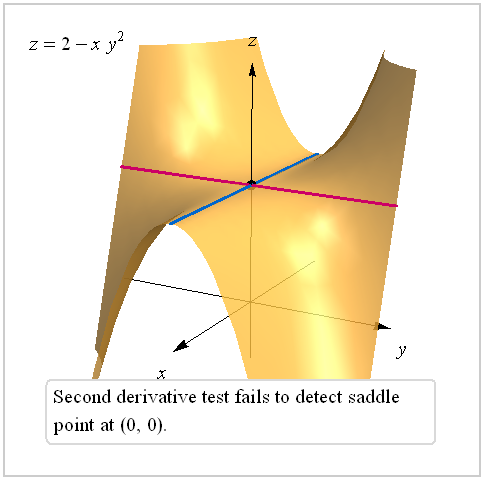
\includegraphics[scale=0.4]{12-8saddle}
\end{center}

%
\framebreak
\begin{center}\tiny
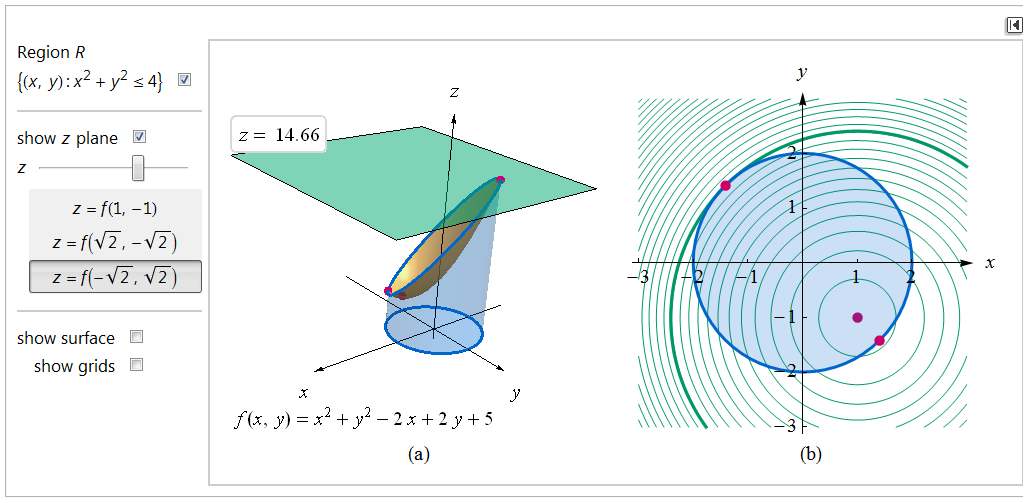
\includegraphics[scale=0.3]{12-8bounded}
\begin{que} What is the parametrization for the boundary? \end{que}
\end{center}
\end{frame}% % %
\subsubsection{Fri 9 Oct}
\begin{frame}{Fri 9 Oct}%\footnotesize
\begin{itemize}
\item No quiz next week but there is one the Thursday after Fall Break.
\item Exam 2 is next week.
	\begin{itemize}
	\item $\sim$7 questions
	\item Get comfortable with ``gnarly" computations.  The best way is to show work while practicing.  See Exam 1 solutions for other shortcuts in work.
	\item No calculators.  
	\item Takehome in drill on Tuesday, covers $\textstyle\oint$12.9.
	\item Expect a list of book problems today.  And look for solutions to Quiz 6.
	\end{itemize}JYH67
\end{itemize}
\end{frame}

% % % % % 
\section{Chapter 13}
\subsection{Week 8}
% % %
\subsubsection{Fri 16 Oct}
\begin{frame}{Fri 16 Oct}%\footnotesize
\begin{itemize}
\item Quiz next week on Thursday.
\item Expect Chapter 13 MLP homeworks posted sometime during Fall Break.
\end{itemize}
\end{frame}

% % % % % 
\subsection{Week 9}
% % %
\subsubsection{Wed 21 Oct}
\begin{frame}{Wed 21 Oct}%\footnotesize
\begin{itemize}
\item Quiz tomorrow: Lagrange multipliers
\item Exam 2 back in drill tomorrow
\item MLP homeworks posted to-nite sometime
\item Friday: 10.2-10.3; Monday: 13.3
\item Final is comprehensive (see syllabus)
\end{itemize}
\end{frame}

% % %
\subsubsection{Fri 23 Oct}
\begin{frame}{Fri 23 Oct}%\small
\begin{itemize}
\item TakeHome Problem...
\item Exam 2 Medians
	\begin{center}
	\includegraphics[scale=0.5]{exam2Medians}
	\end{center}
\item MLP homeworks posted 
\item Monday: 13.3
\item Exam 3 Fri 6 Nov (in 2 weeks) covers Chapter 13
\item Final is comprehensive (see syllabus)
\end{itemize}
\end{frame}

% % % % % 
\subsection{Week 10}
% % %
\subsubsection{Mon 26 Oct}
\begin{frame}{Mon 26 Oct}%\footnotesize
\begin{itemize}
\item Quiz tomorrow... likely on 13.1-2-1
\item stay tuned for Exam 2 solutions
\item Exam 3 Fri 6 Nov (in 2 weeks) covers Chapter 13
\item Final is comprehensive (see syllabus)
\end{itemize}
\end{frame}

% % %
\subsubsection{Fri 30 Oct}
\begin{frame}{Fri 30 Oct}%\small
\begin{itemize}
%\item TakeHome Problem...
\item Exam 2 Medians (curve TBD)
	\begin{center}
	\includegraphics[scale=0.5]{exam2Medians}
	\end{center}
\item MLP homeworks posted -- no 13.6
%\item Monday: 13.3
\item Exam 3 Fri 6 Nov (in 1 week) covers Chapter 13
\item Practice Problems are posted
\item Quiz next week is 13.7-heavy.
\item Final is comprehensive (see syllabus)
\end{itemize}
\end{frame}

% % % % % 
\subsection{Week 11}
% % %
\subsubsection{Mon 2 Nov}
\begin{frame}{Mon 2 Nov}%\footnotesize
\begin{itemize}
\item Quiz tomorrow is 13.7-heavy; 13.7 MLP is available
\item points for MLP 13.1, 13.2, 10.2-3: attempt the new version 
\item Exam 3 Fri 6 Nov
\item Practice Problems are posted on Wheeler-page
\item Quiz and Exam 2 solutions to come
\end{itemize}
\end{frame}

% % %
\subsubsection{Wed 4 Nov}
\begin{frame}{Wed 4 Nov}%\footnotesize
\begin{itemize}
\item Practice Problems are posted on Wheeler-page
\item Quiz and Exam 2 solutions are now posted on MLP
\end{itemize}
\end{frame}

% % % % % % % % % % 
\section{Chapter 14}
% % % % % 
\subsection{Week 12}
% % %
\subsubsection{Mon 9 Nov}
\begin{frame}{Mon 9 Nov}%\footnotesize
\begin{itemize}
\item Quiz tomorrow... prepare up to 14.1 
\item Exams are being graded
\end{itemize}
\end{frame}

%
\begin{frame}[allowframebreaks]{\small Pictures!}\footnotesize
\begin{center}
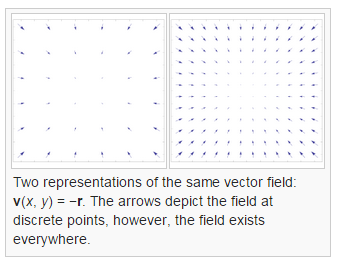
\includegraphics[scale=0.7]{14-1vField}
\end{center}

{\tiny by Connor Glosser - generated with Mathematica 7.0. 
Licensed under Public Domain via Commons} %- \url{https://commons.wikimedia.org/wiki/File:Radial_vector_field_dense.svg#/media/File:Radial_vector_field_dense.svg}
%
\framebreak
\begin{center}
\includegraphics[scale=1.0]{14-1vectorSphere}
\end{center}

{\tiny "Vector sphere" by I, Cronholm144. Licensed under CC BY-SA 3.0 via Commons}% - https://commons.wikimedia.org/wiki/File:Vector_sphere.svg#/media/File:Vector_sphere.svg
\end{frame}

% % %
\subsubsection{Wed 11 Nov}
\begin{frame}{Wed 11 Nov}%\footnotesize
\begin{itemize}
\item Exam 3 medians: stay tuned... test returned in drill tomorrow
\end{itemize}
\end{frame}

% % %
\subsubsection{Fri 13 Nov}
\begin{frame}{Fri 13 Nov}%\footnotesize
\begin{itemize}
\item MakeUp Exams: stay tuned for grading
\item Grading Decisions 
\item Exam 3 medians
\begin{center}
\includegraphics[scale=0.5]{exam3Medians}
\end{center}
\end{itemize}
\end{frame}

% % % % % 
\subsection{Week 13}
% % %
\subsubsection{Mon 16 Nov}
\begin{frame}{Mon 16 Nov}%\footnotesize
\begin{itemize}
\item Quiz tomorrow... prepare up to 14.4
\item MakeUp Exams returned in drill tomorrow
\item Grading Decisions 
\item Exam 3 medians
\begin{center}
\includegraphics[scale=0.5]{exam3Medians}
\end{center}
\end{itemize}
\end{frame}

% % %
\subsubsection{Wed 18 Nov}
\begin{frame}{Wed 18 Nov}%\footnotesize
\begin{itemize}
\item Quiz 11 Thursday 14.2, 14.3
\item Quiz 12 Tuesday 14.4, 14.5
\item Curves are here!
	\begin{itemize}
	\item Exam 2: $\text{New Score}= \textstyle\frac{7}{8}(\alert{\text{Original}}-62)+72$
	\item Exam 3: $\text{New Score}= \textstyle\frac{26}{33}(\alert{\text{Original}}-65)+74$
	\item NO curve in the course.
	\end{itemize}
\item Grading Beefs: Resolve in office hours.
\item Grades are updated.  Except for attendance.
\item Final: Half Chapter 14, half everything else.
\end{itemize}
\end{frame}

% % %
\subsubsection{Fri 20 Nov}
\begin{frame}{Fri 20 Nov}%\footnotesize
\begin{itemize}
\item Quiz 11... study 14.2, 14.3
\item Quiz 12 TBA 14.4, 14.5
\item Curves are here!
	\begin{itemize}
	\item Exam 2: $\text{New Score}= \textstyle\frac{7}{8}(\alert{\text{Original}}-62)+72$
	\item Exam 3: $\text{New Score}= \textstyle\frac{26}{33}(\alert{\text{Original}}-65)+74$
	\item NO curve in the course.
	\end{itemize}
\item Grading Beefs: Resolve in office hours.
\end{itemize}
\end{frame}

% % % % % 
\subsection{Week 14}
% % %
\subsubsection{Mon 23 Nov}
\begin{frame}{Mon 23 Nov}%\footnotesize
\begin{itemize}
\item Quiz 11 tomorrow
\item Quiz 12 Tuesday 14.4, 14.5
\item Exam 3 modified curve: $\text{New Score}= \textstyle\frac{26}{33}(\alert{\text{Original}}-64)+74$
\end{itemize}
\end{frame}

% % % % % 
\subsection{Week 15}
% % %
\subsubsection{Mon 30 Nov}
\begin{frame}{Mon 30 Nov}%\footnotesize
\begin{itemize}
\item Quiz 12 tomorrow 14.4, 14.5: heavier on 14.4
\item Exam 3 modified curve: $\text{New Score}= \textstyle\frac{26}{33}(\alert{\text{Original}}-64)+74$
\item Practice Problems and Formula Sheet are posted
\end{itemize}
\end{frame}

% % %
\subsubsection{Wed 2 Dec}
\begin{frame}{Wed 2 Dec}%\footnotesize
\begin{itemize}
\item MLP assignment due dates from the break will be pushed back, stay tuned...
\item Remainder of the course: 14.7, 14.8.  Read ahead!
\item Tomorrow's drill: sample questions on Stokes' Theorem (14.7)
\item Quiz 13 on Tuesday, covers Divergence Theorem (14.8)
\item Start studying the Practice Problems and Formula Sheet now!
\end{itemize}
\end{frame}

% 
\begin{frame}
\begin{center}
This is Calculus
\vspace{0.5pc}

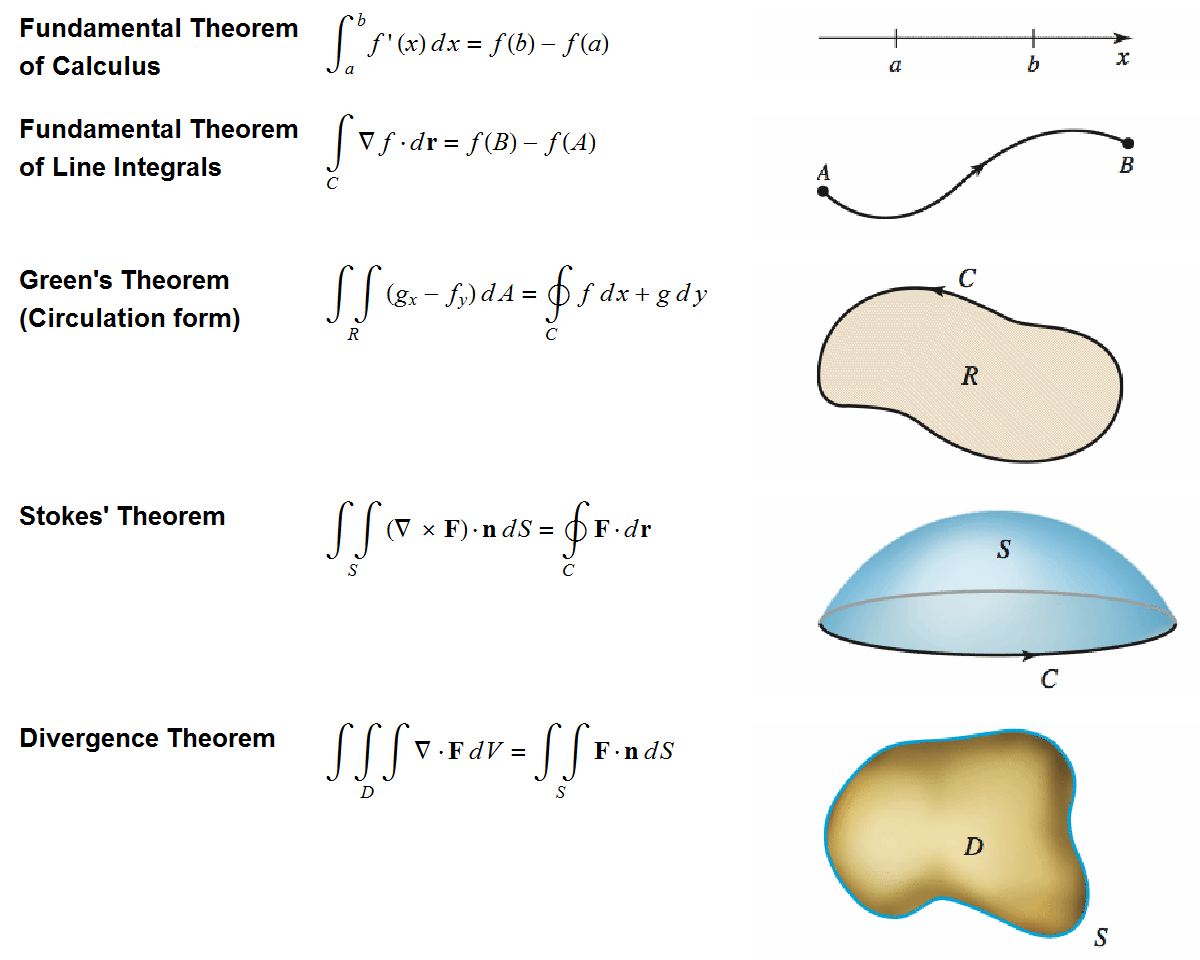
\includegraphics[scale=.5]{fundamentalTheorems}
\end{center}
\end{frame}

% % %
\subsubsection{Fri 4 Dec}
\begin{frame}{Fri 4 Dec}%\footnotesize
\begin{itemize}
\item MLP assignments from the break -- you won't be punished for late submissions from the original due dates 
\item Remainder of the course: 14.7, 14.8.  Read.
\item Quiz 13 on Tuesday, covers Divergence Theorem (14.8) and Stokes' Theorem (14.7)
\item Start studying the Practice Problems and Formula Sheet now!
\end{itemize}
\end{frame}

% 
\begin{frame}
\begin{center}
For use in computing surface integrals.
\vspace{0.5pc}

\includegraphics[scale=.4]{table14-2}
\end{center}
\end{frame}

% 
\begin{frame}
\begin{center}
This is Calculus
\vspace{0.5pc}

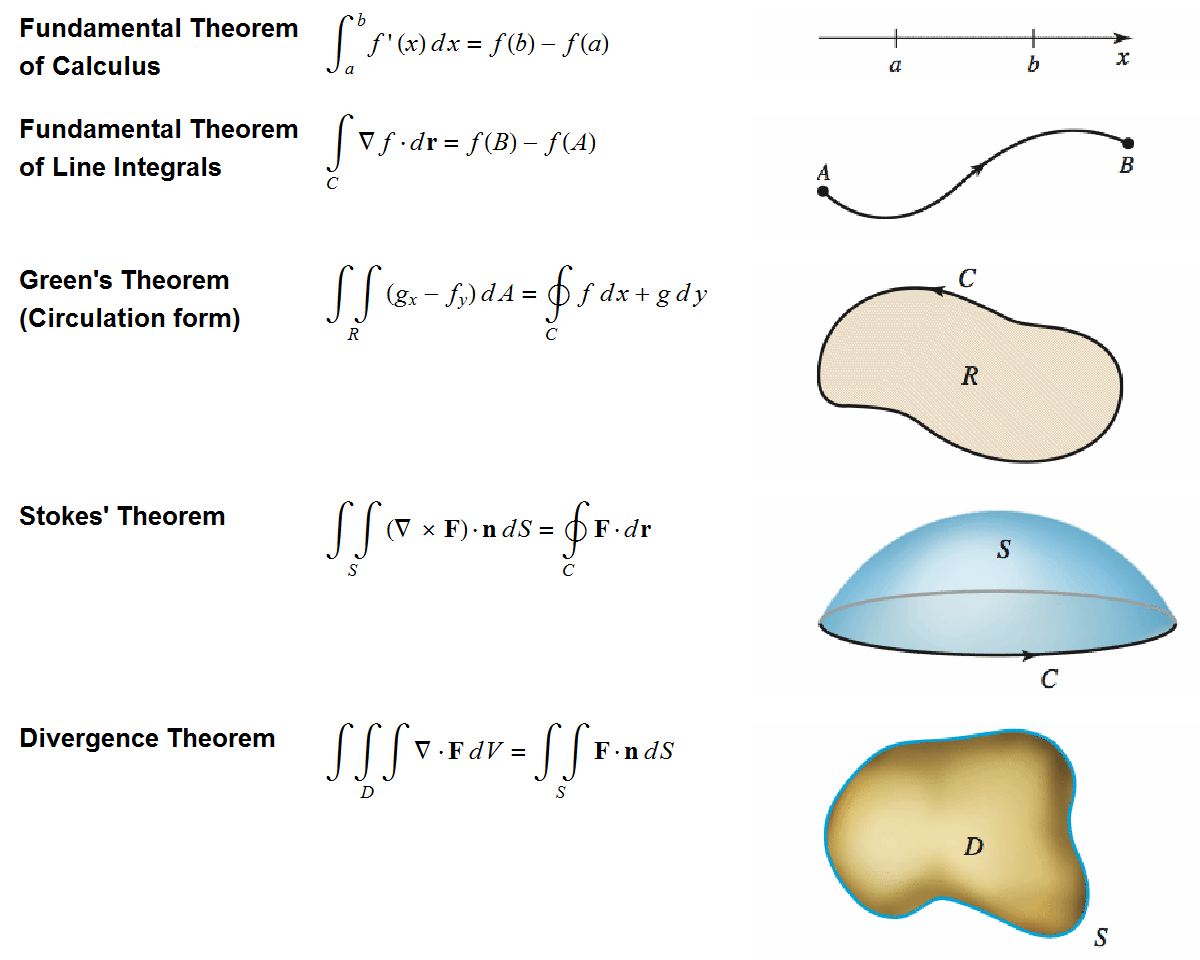
\includegraphics[scale=.5]{fundamentalTheorems}
\end{center}
\end{frame}

% % % % % 
\subsection{Week 16}
% % %
\subsubsection{Mon 7 Dec}
\begin{frame}{Mon 7 Dec}%\footnotesize
\begin{itemize}
\item MLP assignments from the break -- you won't be punished for late submissions from the original due dates 
\item Quiz 13 tomorrow, covers Divergence Theorem (14.8) and Stokes' Theorem (14.7)
\item Start studying the Practice Problems and Formula Sheet NOW.
\end{itemize}
\end{frame}

% 
\begin{frame}
\begin{center}
For use in computing surface integrals.
\vspace{0.5pc}

\includegraphics[scale=.4]{table14-2}
\end{center}
\end{frame}

% 
\begin{frame}
\begin{center}
This is Calculus
\vspace{0.5pc}

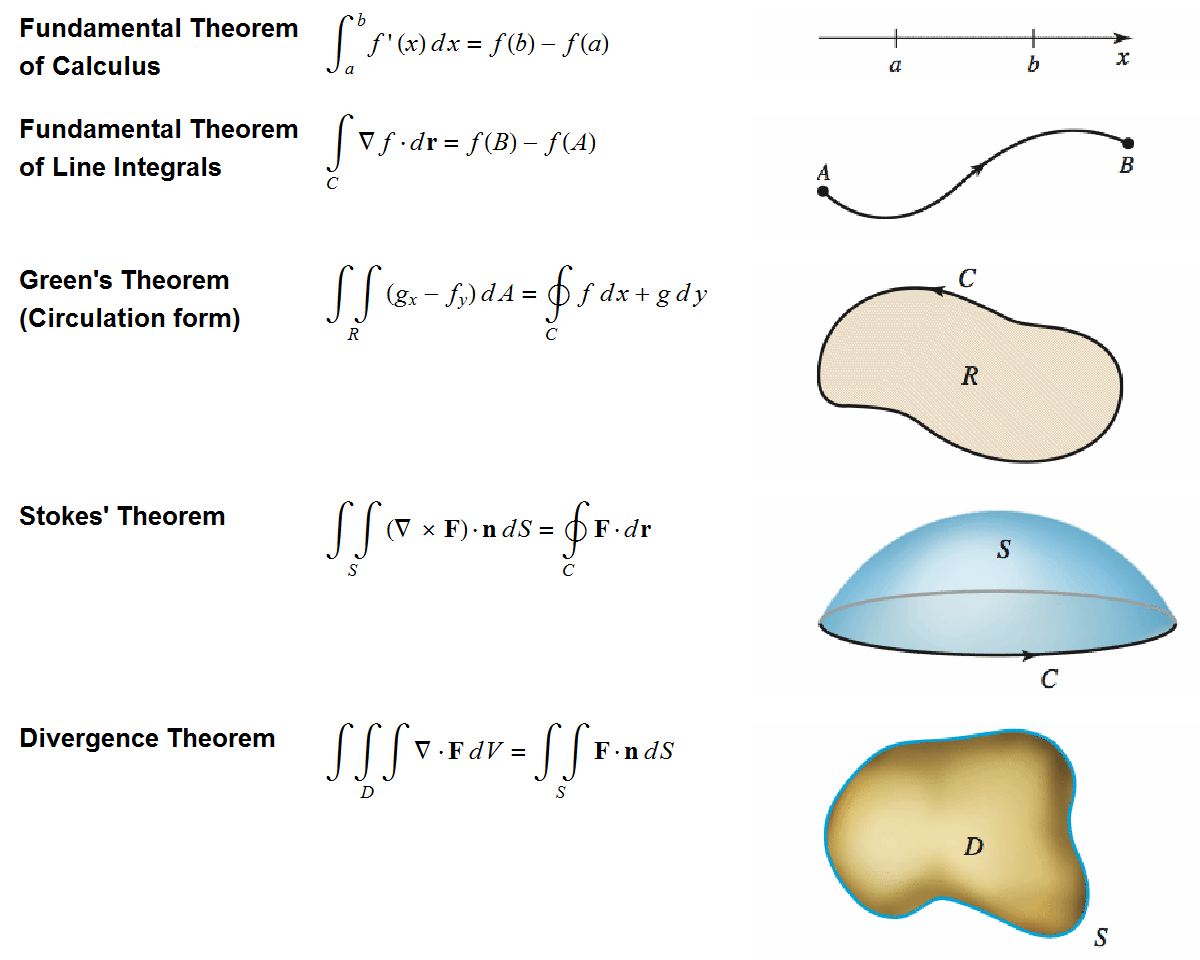
\includegraphics[scale=.5]{fundamentalTheorems}
\end{center}
\end{frame}

% % %
\subsubsection{Wed 9 Dec}
\begin{frame}{Wed 9 Dec}%\footnotesize
\begin{itemize}
\item MLP assignments from the break -- you won't be punished for late submissions from the original due dates 
%\item Quiz 13 tomorrow, covers Divergence Theorem (14.8) and Stokes' Theorem (14.7)
\item Start studying the Practice Problems and Formula Sheet NOW.
\item Stay tuned for more Goodies...
\end{itemize}
\end{frame}

% 
\begin{frame}
\begin{center}
For use in computing surface integrals.
\vspace{0.5pc}

\includegraphics[scale=.4]{table14-2}
\end{center}
\end{frame}

% 
\begin{frame}
\begin{center}
This is Calculus
\vspace{0.5pc}

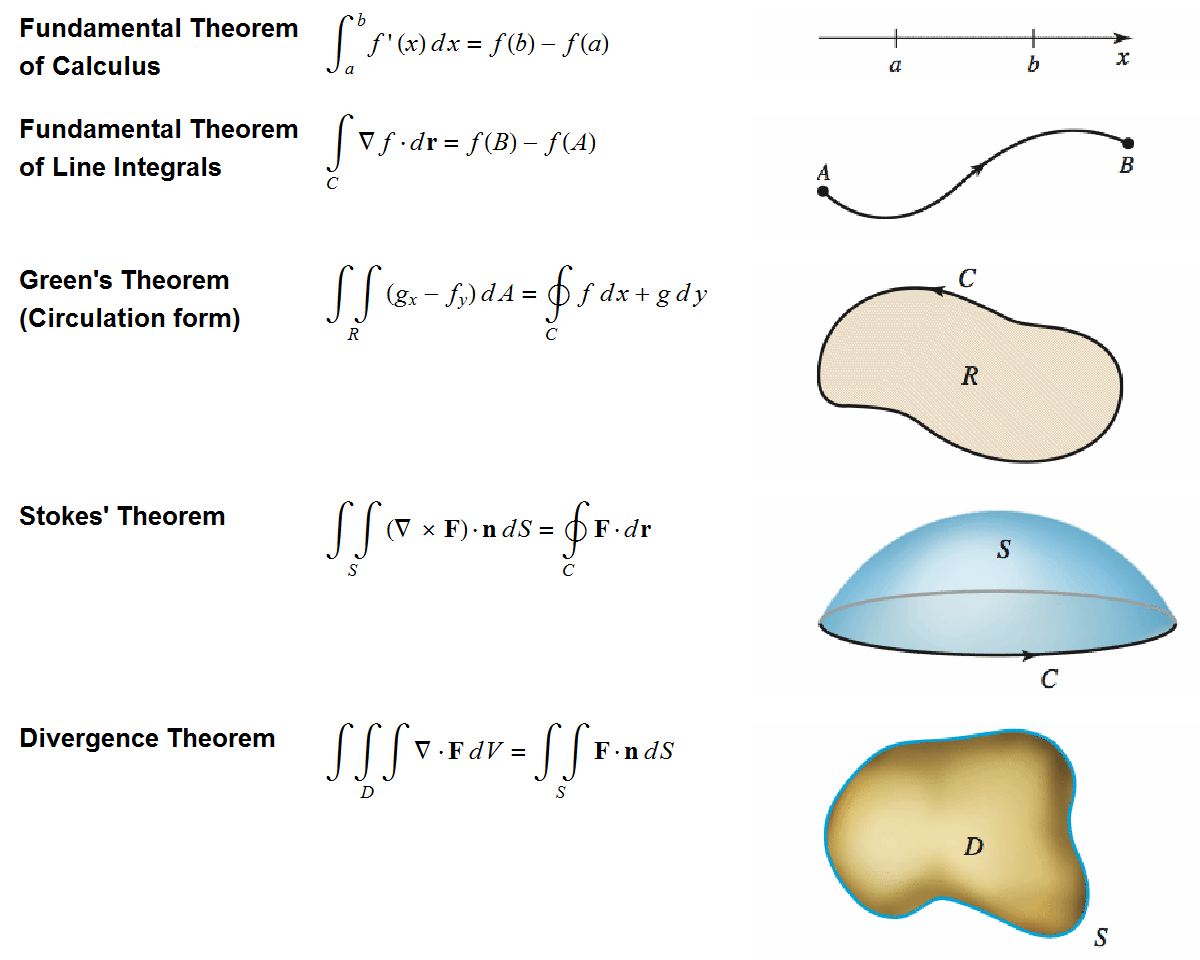
\includegraphics[scale=.5]{fundamentalTheorems}
\end{center}
\end{frame}


\end{document}